OpenId Connect — это дополнительный уровень~\cite{siriwardenaOpenid2020, sakimuraOpenid2014} идентификации поверх
протокола~\cite{hardt2012oauth} OAuth 2.0.
Он позволяет клиентам проверять личность конечного пользователя на основе аутентификации,
а также получать базовую информацию о профиле конечного пользователя.

OAuth 2.0 — это протокол, позволяющий стороннему приложению получить ограниченный доступ к HTTP-сервису, либо от имени
владельца ресурса, организуя взаимодействие по утверждению между владельцем ресурса и HTTP-сервисом, либо путем разрешения
стороннему приложению получить доступ от своего имени.

В традиционной модели аутентификации клиент-сервер, клиент запрашивает ресурс с ограниченным доступом
через аутентификацию с использованием пары логин-пароль.
Для того чтобы предоставить стороннему приложению доступ к ресурсам,
владелец ресурса (пользователь) делится своими учетными данными (логином и паролем) со сторонним приложением.
Этот подход создает ряд проблем и ограничений~\cite{hardt2012oauth}:
\begin{itemize}
    \item Сторонние приложения должны хранить учетные данные (логин и пароль) владельца ресурса для дальнейшего использования,
    бывает так, что пароль хранится в явном виде в базе данных.
    \item Сторонние приложения обязаны поддерживать аутентификацию с помощью пароля, несмотря на недостатки безопасности,
    присущие паролям.
    \item Сторонние приложения получают полный доступ к защищенным ресурсам владельца ресурса (пользователя),
    оставляя владельцев ресурсов без какой-либо возможности ограничить продолжительность доступа или подмножество
    доступных ресурсов (scope).
    \item Владельцы ресурсов (пользователи) не могут отозвать доступ к отдельному третьему лицу без отзыва доступа для всех
    третьих лиц, и должны отозвать доступ только путем изменения пароля.
    \item Взлом либо утечка данных из любого стороннего приложения приводит к потере пароля конечного пользователя и
    всех данных, защищенных этим паролем.
\end{itemize}

OAuth 2.0 решает эти проблемы путем введения уровня авторизации и разделения роли клиента (сервис авторизации) и
владельца ресурса (пользователя).
В OAuth 2.0 клиент запрашивает доступ к ресурсам, контролируемым владельцем ресурса и размещенным на сервере ресурса.
Вместо того чтобы использовать учетные данные владельца ресурса для доступа к защищенным ресурсам, клиент получает токен доступа.

OAuth 2.0 with the Proof of Key Code Exchange~\cite{bradley2015rfc} flow показан ниже
\begin{figure}[H]
    \centering
    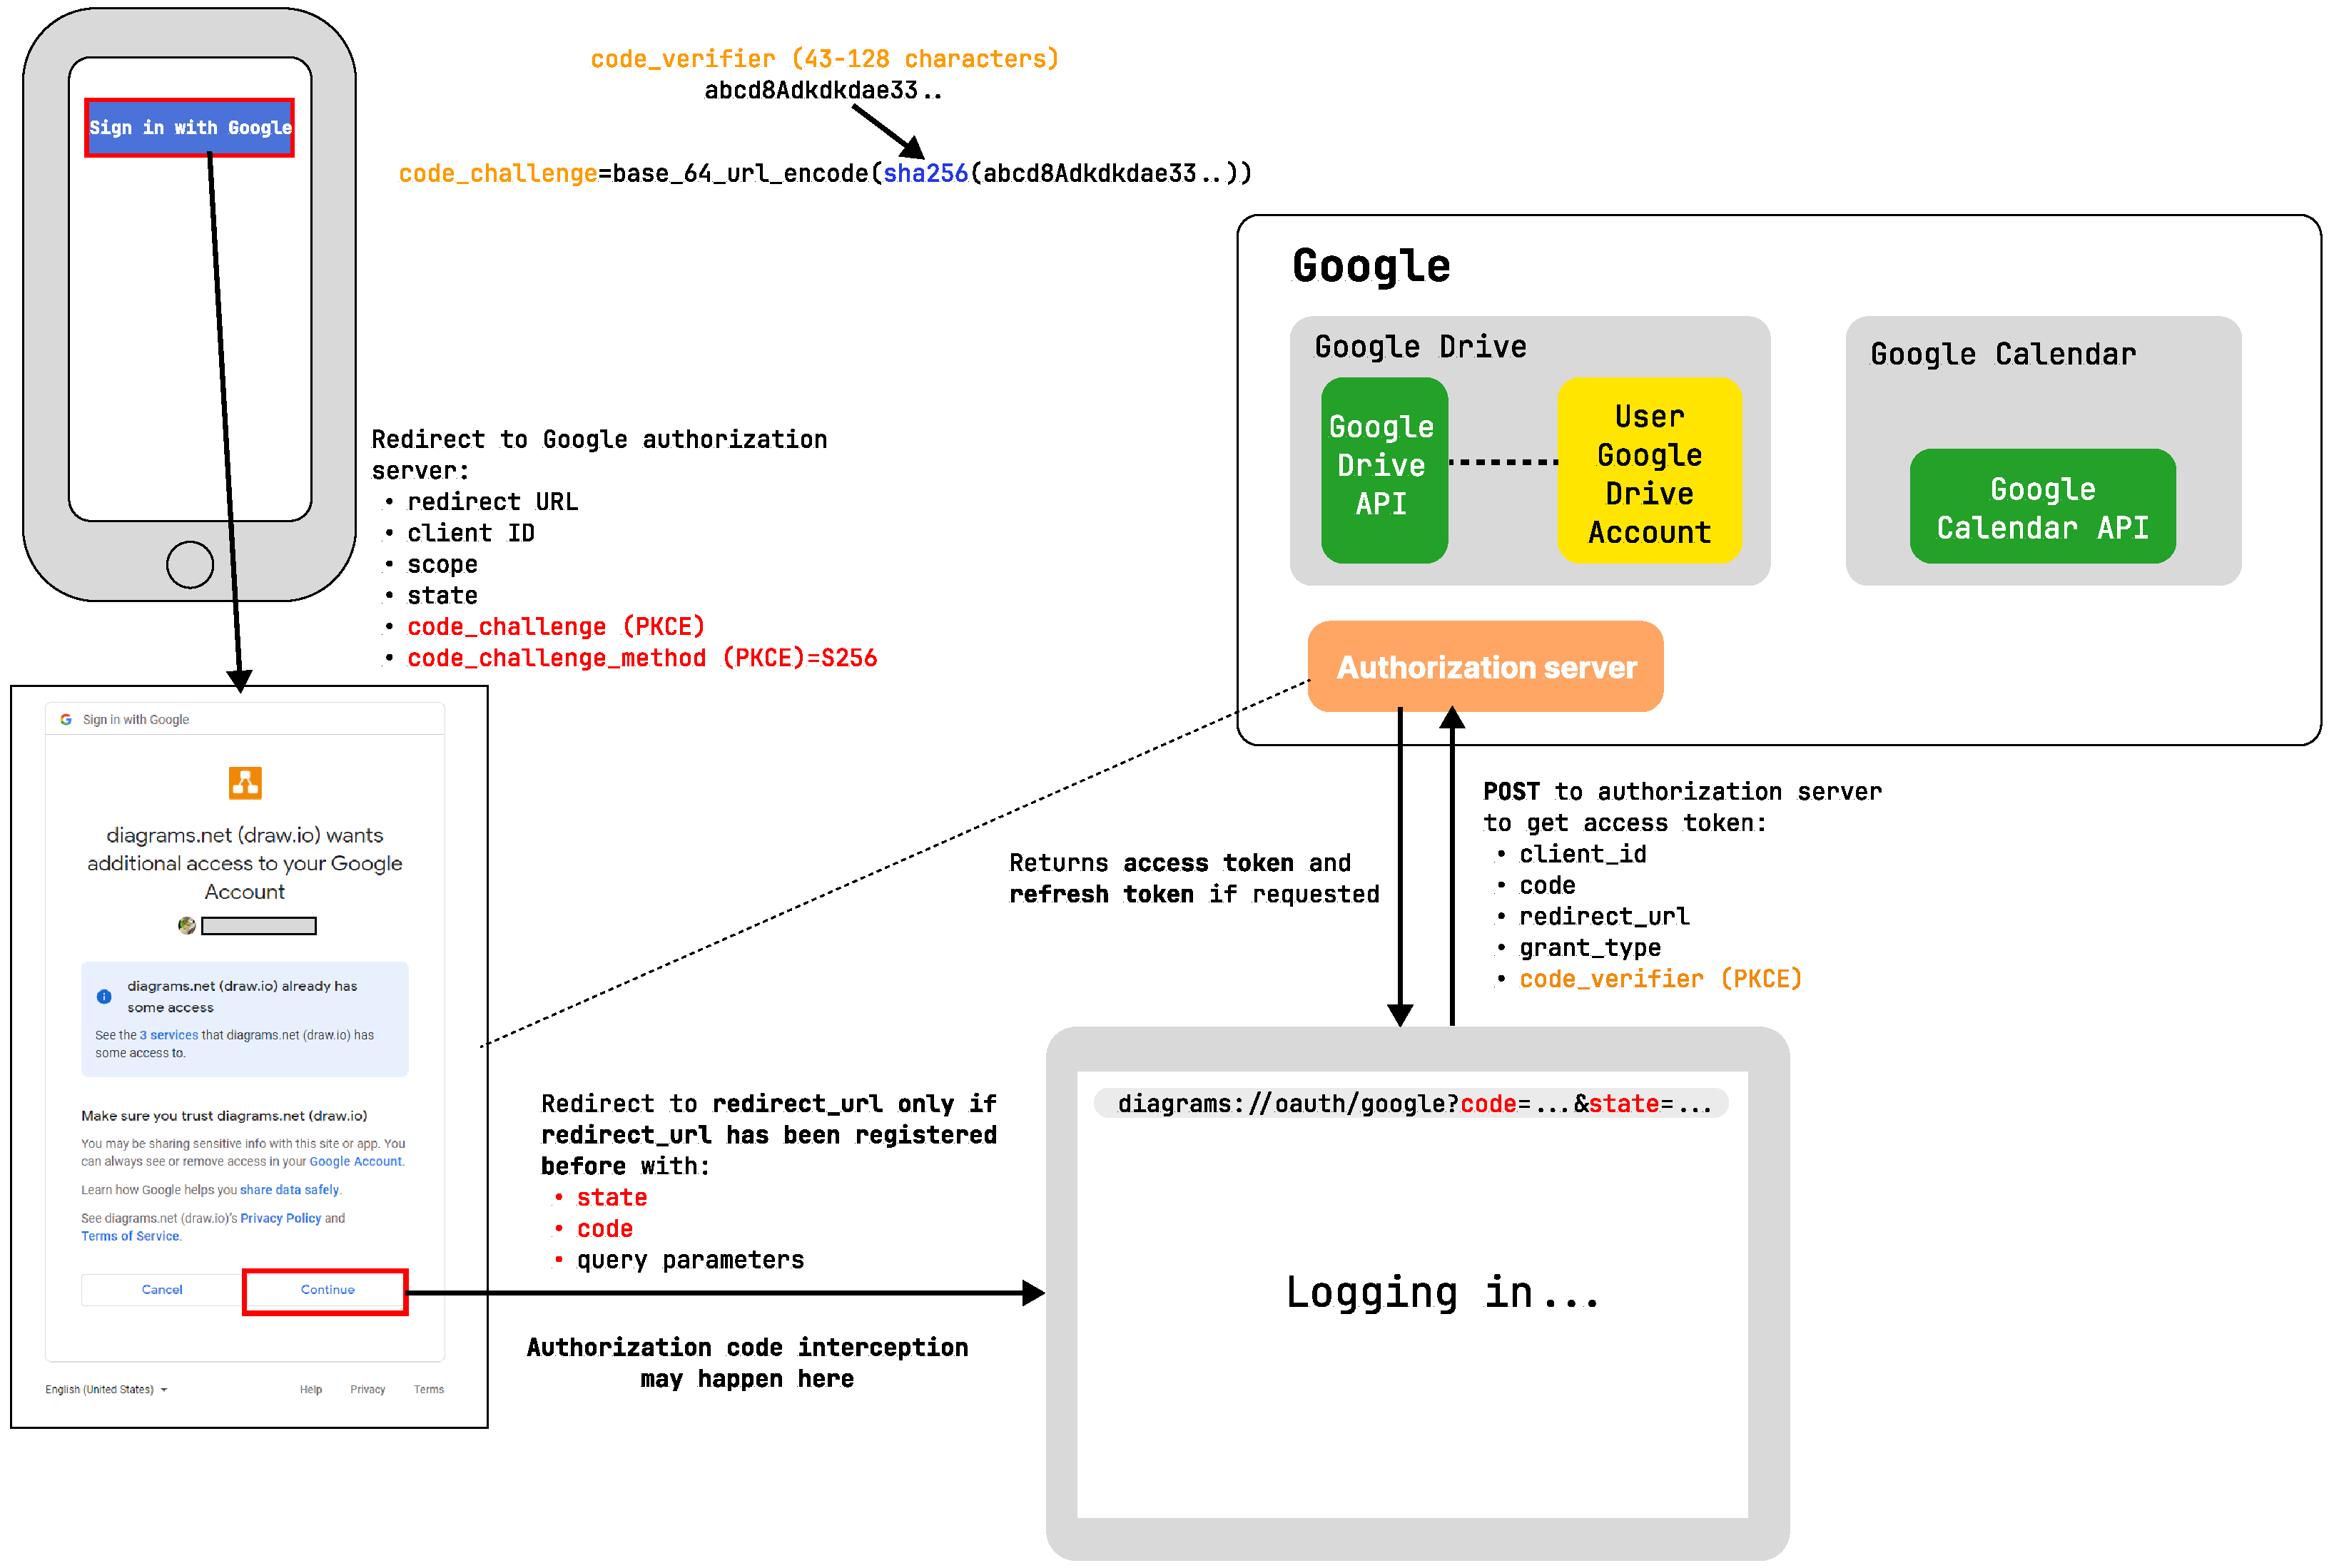
\includegraphics[width=1\textwidth]{img/OAuthPkceScheme_1570_1055}
    ~\caption{OAuth 2.0 with PKCE flow diagram.}\label{fig:figure2}
\end{figure}

\begin{enumerate}
    \item После нажатия на кнопку \texttt{Sign in with Google} происходит перенаправление на ендпоинт авторизации,
    на котором владелец ресурса должен ввести свои учетные данные, а так же согласиться с некоторыми условиями.
    Особое внимание стоит обратить на code\_challenge и code\_challenge\_method, первое представляет собой некоторую строку,
    которая будет закодирована с помощью метода кодировки указанного в параметре запроса code\_challenge\_method.
    В дальнейшем, при обмене полученного кода на токен доступа и обновления, мы должны будем предъявить значение code\_verifier,
    которое равно ранее закондированному code\_challenge.
    \item После успешной аутентификации, произойдет перенаправление на адресс \texttt{redirect\_uri}.
    \item После получения авторизационного кода происходит обмен этого кода на токены доступа (access token) и
    обновления (refresh token).
    Если ранее, при переадресации владельца ресурса на авторизационный ендпоинт, мы указывали \texttt{code\_challenge}
    и \texttt{code\_challenge\_method},
    то теперь, при обмене кода на токены, мы обязаны передать в запросе значение \texttt{code\_verifier}.
\end{enumerate}
Здесь мы упоминаем такие определения, как code и state.
\begin{itemize}
    \item \textbf{Code} - это код авторизации, который получается с помощью сервера авторизации и является посредником
    между клиентов и владельцем ресурса.
    Перед тем как сервер авторизации перенаправит владельца ресурса обратно на клиент, сервер авторизации проверяет
    подлинность владельца ресурса.
    Так образом поскольку владелец ресурса аутентифицируется только на сервере авторизации, его учетные данные никогда
    не передадутся клиенту.
    \item \textbf{State} - значение, используемое клиентом для сохранения состояния между запросом на авторизацию и
    обратным вызовом (callback).
    Сервер авторизации включает это значение при перенаправлении агента пользователя обратно клиенту.
    Этот параметр используется для предотвращения Cross-Site Request Forgery (CSRF) атак.
\end{itemize}

Authorization code flow with PKCE является протоколом, который представляет секрет, созданный клиентом,
который может быть проверен сервером авторизации.
Этот секрет называется \texttt{code\_verifier}.
Клиент хеширует значение \texttt{code\_verifier} и записывает его в параметр \texttt{code\_challenge}.
PKCE решает проблему безопасного обмена кода.
Если злоумышленнику удастся заполучить авторизационный код, то у него не получится обменять
его на токены доступа и обновления.
Таким образом, мы гарантируем тот факт, что обмен кода на токены производит то же самое приложение, что и выполняло
аутентификацию.
В некотором роде, PKCE можно сравнить с цифровой подписью процесса аутентификации.
При обмене кода авторизации на токены обязательно нужно указать \texttt{code\_verifier}.